% =============================================================================
% Sparse FFN | MVS Project | NIT Mizoram — Professional Beamer Presentation
% Authors : Lakshmi Ganapathi Kodi (BT23MA005) & Saurabh Kumar Gupta (BT23MA006)
% Compile : pdflatex  (run twice for page numbers)
% =============================================================================
\documentclass[aspectratio=169,10pt]{beamer}

% ---- packages ----------------------------------------------------------------
\usetheme{default}
\usefonttheme{professionalfonts}
\usepackage[T1]{fontenc}
\usepackage{lmodern}
\usepackage{amsmath,amssymb,mathtools,bm}
\usepackage{graphicx}
\usepackage{booktabs,tabularx,array,multirow}
\usepackage{ragged2e}
\usepackage{tikz}
\usetikzlibrary{positioning,arrows.meta,calc,shapes.geometric,fit}
\usepackage{hyperref}
\hypersetup{colorlinks=false}
\usepackage{microtype}

% ---- colour palette (Deep Navy / Gold academic theme) -----------------------
\definecolor{NavyDeep}{HTML}{0A1628}   % primary dark – titles, header bg
\definecolor{NavyMid} {HTML}{1A3A6B}   % secondary navy – block titles
\definecolor{Gold}    {HTML}{C8922A}   % accent gold
\definecolor{GoldLight}{HTML}{F5D78E}  % soft gold tint
\definecolor{IceBlue} {HTML}{EEF3FB}   % body block bg
\definecolor{Crimson} {HTML}{C0392B}   % alert / emphasis
\definecolor{CrimsonTint}{HTML}{FDECEA}
\definecolor{SlateGray}{HTML}{2D3748}  % main body text
\definecolor{Muted}   {HTML}{5A6880}   % captions / notes
\definecolor{LineGray}{HTML}{CBD5E0}   % rule lines
\definecolor{PaperBg} {HTML}{F8F9FC}   % slide background

% ---- beamer colour assignments ----------------------------------------------
\setbeamercolor{normal text}        {fg=SlateGray,     bg=PaperBg}
\setbeamercolor{structure}          {fg=NavyMid}
\setbeamercolor{frametitle}         {fg=white,         bg=NavyDeep}
\setbeamercolor{title}              {fg=white}
\setbeamercolor{subtitle}           {fg=GoldLight}
\setbeamercolor{block title}        {fg=white,         bg=NavyMid}
\setbeamercolor{block body}         {fg=SlateGray,     bg=IceBlue}
\setbeamercolor{alertblock title}   {fg=white,         bg=Crimson}
\setbeamercolor{alertblock body}    {fg=SlateGray,     bg=CrimsonTint}
\setbeamercolor{exampleblock title} {fg=white,         bg=NavyDeep}
\setbeamercolor{exampleblock body}  {fg=SlateGray,     bg=IceBlue}
\setbeamercolor{itemize item}       {fg=Gold}
\setbeamercolor{itemize subitem}    {fg=NavyMid}
\setbeamercolor{enumerate item}     {fg=NavyMid}
\setbeamercolor{footline}           {fg=white,         bg=NavyDeep}
\setbeamercolor{takeaway}           {fg=white,         bg=NavyMid}

% ---- beamer font assignments ------------------------------------------------
\setbeamerfont{title}      {size=\Large,series=\bfseries}
\setbeamerfont{subtitle}   {size=\normalsize}
\setbeamerfont{frametitle} {size=\large,series=\bfseries}
\setbeamerfont{block title}{series=\bfseries}

% ---- bullet items -----------------------------------------------------------
\setbeamertemplate{navigation symbols}{}
\setbeamertemplate{itemize item}{%
  \raise0.15ex\hbox{\scriptsize\color{Gold}$\blacktriangleright$}}
\setbeamertemplate{itemize subitem}{%
  \raise0.1ex\hbox{\tiny\color{NavyMid}$\blacktriangleright$}}
\setbeamertemplate{enumerate item}{\color{NavyMid}\insertenumlabel.}

% ---- custom frame title -----------------------------------------------------
\setbeamertemplate{frametitle}{%
  \nointerlineskip%
  \begin{beamercolorbox}[wd=\paperwidth,ht=0.68cm,dp=0.14cm,%
      leftskip=0.5cm,rightskip=0.42cm]{frametitle}%
    \usebeamerfont{frametitle}\insertframetitle%
    \hfill{\color{GoldLight}\scriptsize\insertsection}%
  \end{beamercolorbox}%
  % thin gold rule under header
  {\color{Gold}\rule{\paperwidth}{0.8pt}}%
}

% ---- footline ---------------------------------------------------------------
\setbeamertemplate{footline}{%
  \leavevmode%
  \hbox{%
    \begin{beamercolorbox}[wd=.72\paperwidth,ht=2.5ex,dp=1ex,leftskip=.45cm]{footline}%
      \scriptsize\color{white}%
      Sparse FFN $\mid$ NIT Mizoram%
      \hspace{0.8em}{\color{Gold}\textbullet}\hspace{0.5em}%
      Multivariate Statistical Analysis
    \end{beamercolorbox}%
    \begin{beamercolorbox}[wd=.28\paperwidth,ht=2.5ex,dp=1ex,rightskip=.45cm plus1fil]{footline}%
      \scriptsize\color{white}\hfill\insertframenumber\,/\,\inserttotalframenumber
    \end{beamercolorbox}%
  }%
}

% ---- spacing & layout -------------------------------------------------------
\setbeamersize{text margin left=0.5cm,text margin right=0.5cm}
\setlength{\abovedisplayskip}{3pt}
\setlength{\belowdisplayskip}{3pt}
\setlength{\abovedisplayshortskip}{1pt}
\setlength{\belowdisplayshortskip}{1pt}
\renewcommand{\arraystretch}{1.10}

% ---- helper macros ----------------------------------------------------------
\newcommand{\metricbox}[3]{%
  \begin{beamercolorbox}[wd=\linewidth,rounded=true,sep=5pt,center]{block body}%
    {\color{NavyMid}\Large\bfseries #1}\par\vspace{1pt}%
    {\footnotesize\bfseries #2}\par%
    {\scriptsize\color{Muted}#3}%
  \end{beamercolorbox}%
}
\newcommand{\takeaway}[1]{%
  \vspace{3pt}%
  \begin{beamercolorbox}[wd=\linewidth,rounded=true,sep=5pt]{takeaway}%
    {\small\bfseries\color{GoldLight}KEY TAKEAWAY}%
    \par\vspace{2pt}{\small #1}%
  \end{beamercolorbox}%
}
\newcommand{\rqbadge}[1]{%
  \tikz[baseline=(x.base)]\node[%
    rounded corners=2pt,fill=Gold,text=NavyDeep,%
    inner xsep=5pt,inner ysep=2pt,font=\bfseries\scriptsize](x){#1};%
}
\newcommand{\smallnote}[1]{{\scriptsize\color{Muted}#1}}
\newcommand{\Hnull}{\mathcal{H}_0}
\newcommand{\erank}{\operatorname{erank}}
\newcommand{\PR}{\operatorname{PR}}
\newcommand{\ReLU}{\operatorname{ReLU}}
\newcommand{\I}{\mathbb{I}}
\newcommand{\R}{\mathbb{R}}

% ---- title metadata ---------------------------------------------------------
\title{Statistical Characterisation of Sparse Activations and\\[2pt]
       Low-Rank Latent Structures in Dense Feed-Forward Networks}
\subtitle{A Multivariate Statistical Study of OPT-125M on WikiText-2}
\author{Lakshmi Ganapathi Kodi \texttt{(BT23MA005)} \and
        Saurabh Kumar Gupta \texttt{(BT23MA006)}}
\institute{Department of Mathematics, National Institute of Technology Mizoram}
\date{November 2026}

% =============================================================================
\begin{document}
% =============================================================================

% ---- background for all slides ----------------------------------------------
\setbeamertemplate{background}{%
  \begin{tikzpicture}[remember picture,overlay]
    \fill[PaperBg] (current page.south west) rectangle (current page.north east);
    \fill[NavyDeep,opacity=0.04]
      ([xshift=-1cm,yshift=-1cm]current page.north east) circle (5cm);
  \end{tikzpicture}%
}

% =============================================================================
% SLIDE 1 — TITLE
% =============================================================================
\begin{frame}[plain]
\begin{tikzpicture}[remember picture,overlay]
  % full dark header band
  \fill[NavyDeep]
    (current page.north west) rectangle
    ([yshift=-3.8cm]current page.north east);
  % thin gold rule below header
  \fill[Gold]
    ([yshift=-3.8cm]current page.north west) rectangle
    ([yshift=-3.95cm]current page.north east);
  % decorative corner triangle
  \fill[Gold,opacity=0.25]
    (current page.north east) --
    ([xshift=-3.5cm]current page.north east) --
    (current page.north east|-[yshift=-3.8cm]current page.north east) -- cycle;
  % bottom accent dots
  \fill[Gold]  ([xshift=0.4cm,yshift=0.4cm]current page.south west) circle (0.1cm);
  \fill[NavyMid] ([xshift=0.75cm,yshift=0.4cm]current page.south west) circle (0.1cm);
\end{tikzpicture}

\vspace{0.4cm}
{\color{GoldLight}\small\bfseries CSP 1602 \quad|\quad MULTIVARIATE STATISTICAL ANALYSIS}\par
\vspace{0.5cm}
{\color{white}\large\bfseries Statistical Characterisation of Sparse Activations and%
 Low-Rank Latent Structures\\[2pt] in Dense Feed-Forward Neural Networks}\par
\vspace{0.18cm}
{\color{GoldLight}\normalsize Layer dynamics, neuron dependence, intrinsic dimensionality and domain sensitivity}\par

\vspace{0.85cm}
\begin{columns}[c,onlytextwidth]
\column{.68\textwidth}
\centering
{\normalsize\bfseries Lakshmi Ganapathi Kodi}\quad{\small(BT23MA005)}\\[2pt]
{\normalsize\bfseries Saurabh Kumar Gupta}\quad{\small(BT23MA006)}\\[0.5cm]
{\small\color{white}Under the external guidance of}\par
{\normalsize\bfseries\color{white}Prof. Ashis SenGupta}\\[1pt]
{\small\color{white}Applied Statistics Unit, Indian Statistical Institute, Kolkata}\par
\vspace{0.25cm}
{\small\color{white}Internal Guide: Dr. C Lalengmawia, Dept. of CSE, NIT Mizoram}\par
\vspace{0.25cm}
{\small\color{GoldLight}Department of Mathematics $\mid$ NIT Mizoram $\mid$ November 2026}
\column{.28\textwidth}
\centering

\includegraphics[width=2.6cm,keepaspectratio]{assets/nit_logo.png}
\end{columns}
\end{frame}

% =============================================================================
% SLIDE 2 — ROADMAP
% =============================================================================
\section{Overview}
\begin{frame}{Presentation Roadmap}
\begin{columns}[T,onlytextwidth]
\column{.48\textwidth}
\begin{block}{FOUNDATION}
\begin{enumerate}
  \item Motivation and problem statement
  \item Project objectives and research hypotheses
  \item Model, dataset and activation pipeline
\end{enumerate}
\end{block}
\vspace{3pt}
\begin{block}{STATISTICAL FORMULATION}
\begin{enumerate}\setcounter{enumi}{3}
  \item RQ1: Layer-wise sparsity profile
  \item RQ2: Neuron co-activation structure
  \item RQ3: Latent intrinsic dimensionality
\end{enumerate}
\end{block}
\column{.49\textwidth}
\begin{block}{EMPIRICAL EVIDENCE}
\begin{enumerate}\setcounter{enumi}{6}
  \item RQ4: Static weights vs.\ dynamic activations
  \item RQ5: Cross-domain representation invariance
  \item Integrated findings and architectural interpretation
\end{enumerate}
\end{block}
\vspace{3pt}
\begin{alertblock}{CLOSING}
Conclusion, limitations, future directions, and open discussion.
\end{alertblock}
\end{columns}
\end{frame}

% =============================================================================
% SLIDE 3 — MOTIVATION
% =============================================================================
\begin{frame}{Motivation: The Dense-Weight / Sparse-Activation Paradox}
\begin{columns}[T,onlytextwidth]
\column{.56\textwidth}
\begin{block}{Why focus on Transformer FFNs?}
\begin{itemize}
  \item FFN sub-layers hold the majority of parameters and computation in Transformers.
  \item In OPT-125M, each token representation expands from $d=768$ to $d_{ff}=3{,}072$.
  \item ReLU sets every negative pre-activation to an \emph{exact} zero.
  \item Weight matrices remain dense even when most intermediate neurons are inactive.
\end{itemize}
\end{block}
\takeaway{The project asks: how much of the nominal 3{,}072-dimensional FFN space is \emph{actually} used, how does it vary with depth, and what structure underlies the active features?}
\column{.40\textwidth}
\metricbox{768}{Model width $d_{\mathrm{model}}$}{Input token representation}
\vspace{5pt}
\metricbox{3,072}{FFN width $d_{ff}$}{Intermediate feature space}
\vspace{5pt}
\metricbox{12}{Transformer layers}{OPT-125M decoder stack}
\end{columns}
\end{frame}

% =============================================================================
% SLIDE 4 — FFN EQUATION + RESEARCH QUESTIONS TABLE
% =============================================================================
\begin{frame}{FFN Computation and Five Research Questions}
\begin{block}{Feed-forward computation in each Transformer layer $\ell$}
\begin{equation}
  \mathbf{h}^{(\ell)}=\ReLU\!\bigl(\mathbf{x}^{(\ell)}\mathbf{W}_1^{(\ell)}+\mathbf{b}_1^{(\ell)}\bigr),
  \qquad
  \mathbf{y}^{(\ell)}=\mathbf{h}^{(\ell)}\mathbf{W}_2^{(\ell)}+\mathbf{b}_2^{(\ell)}.
  \label{eq:ffn}
\end{equation}
\end{block}
\small
\begin{tabularx}{\linewidth}{>{\bfseries}p{0.07\linewidth} X X}
\toprule
RQ & Research Question & Null Hypothesis (summary)\\
\midrule
RQ1 & Is sparsity constant across the 12 layers? & $\mu_0=\mu_1=\cdots=\mu_{11}$\\
RQ2 & Do neurons co-activate or fire independently? & $\phi_{ij}=0$ for all $i\ne j$\\
RQ3 & Is the activation space full-dimensional? & $\erank(\mathbf{S})=3{,}072$\\
RQ4 & Do weight and activation ranks track each other? & Static and dynamic ranks are directly coupled\\
RQ5 & Are activation manifolds domain-invariant? & $\boldsymbol\mu_{\mathrm{wiki}}=\boldsymbol\mu_{\mathrm{sci}}=\boldsymbol\mu_{\mathrm{news}}$\\
\bottomrule
\end{tabularx}
\vspace{3pt}
\smallnote{Individual test assumptions and estimands are described on each RQ slide.}
\end{frame}

% =============================================================================
% SLIDE 5 — PIPELINE
% =============================================================================
\begin{frame}{Experimental Architecture: From Text to Statistical Evidence}
\centering
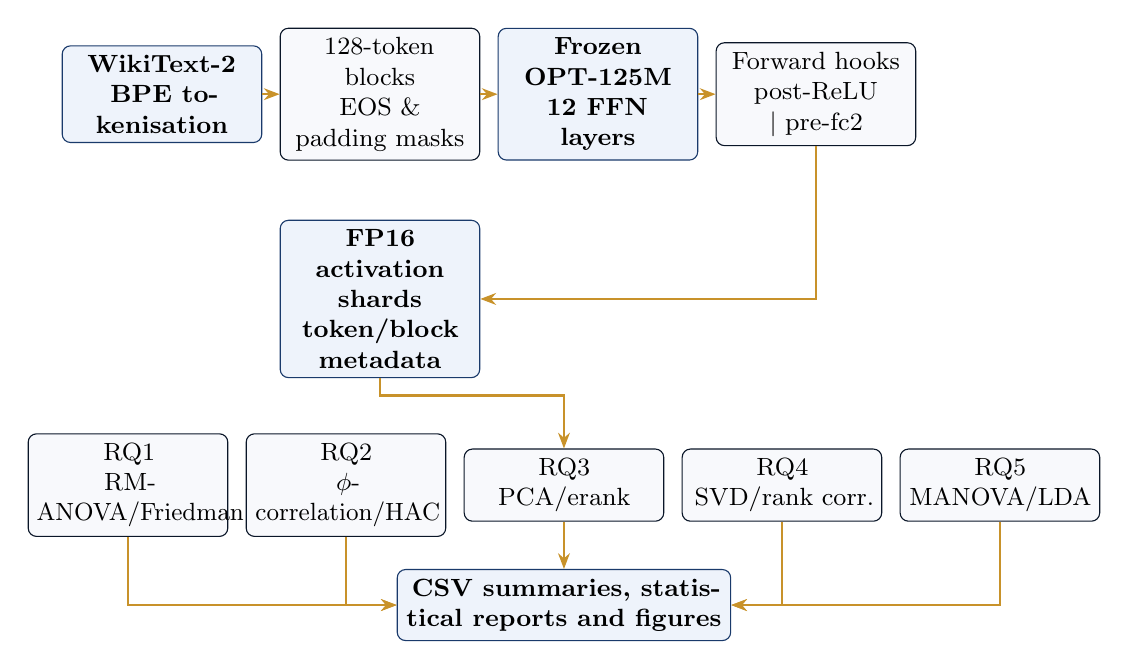
\begin{tikzpicture}[
  node distance=0.4cm and 0.22cm,
  stage/.style={rounded corners=3pt,draw=NavyMid,fill=IceBlue,minimum height=0.84cm,
                text width=2.3cm,align=center,font=\small\bfseries},
  proc/.style ={rounded corners=3pt,draw=NavyDeep,fill=PaperBg,minimum height=0.84cm,
                text width=2.3cm,align=center,font=\small},
  arr/.style  ={-{Stealth[length=2mm]},thick,color=Gold}
]
\node[stage] (data)  {WikiText-2\\BPE tokenisation};
\node[proc,  right=of data]   (chunks){128-token blocks\\EOS \& padding masks};
\node[stage, right=of chunks] (model) {Frozen OPT-125M\\12 FFN layers};
\node[proc,  right=of model]  (hooks) {Forward hooks\\post-ReLU $\mid$ pre-fc2};
\draw[arr] (data)--(chunks); \draw[arr] (chunks)--(model); \draw[arr] (model)--(hooks);
\node[stage,below=0.75cm of chunks] (store) {FP16 activation shards\\token/block metadata};
\draw[arr] (hooks.south) |- (store.east);
\node[proc,below=0.7cm of store,xshift=-3.2cm] (rq1) {RQ1\\RM-ANOVA/Friedman};
\node[proc,right=0.22cm of rq1] (rq2) {RQ2\\$\phi$-correlation/HAC};
\node[proc,right=0.22cm of rq2] (rq3) {RQ3\\PCA/erank};
\node[proc,right=0.22cm of rq3] (rq4) {RQ4\\SVD/rank corr.};
\node[proc,right=0.22cm of rq4] (rq5) {RQ5\\MANOVA/LDA};
\draw[arr] (store.south) -- ++(0,-0.22) -| (rq3.north);
\node[stage,below=0.6cm of rq3,text width=4.0cm]
  (out) {CSV summaries, statistical reports and figures};
\draw[arr] (rq1.south) |- (out.west);
\draw[arr] (rq2.south) |- (out.west);
\draw[arr] (rq3.south) -- (out.north);
\draw[arr] (rq4.south) |- (out.east);
\draw[arr] (rq5.south) |- (out.east);
\end{tikzpicture}
\end{frame}

% =============================================================================
% SLIDE 6 — DATASET / ACTIVATION EXTRACTION
% =============================================================================
\begin{frame}{Dataset and Activation Extraction}
\begin{columns}[T,onlytextwidth]
\column{.50\textwidth}
\begin{block}{Text processing}
\begin{itemize}
  \item Primary corpus: Salesforce WikiText-2 raw-v1.
  \item OPT-125M byte-pair encoding tokenizer.
  \item End-of-sequence marker preserved between source rows.
  \item Non-overlapping contiguous blocks of length $L=128$.
  \item Padding positions are tracked and excluded from summaries.
\end{itemize}
\end{block}
\column{.47\textwidth}
\begin{block}{Activation capture}
\begin{equation}
\mathbf{H}^{(\ell)}=\ReLU\!\bigl(\mathrm{fc1}^{(\ell)}(\mathbf{X}^{(\ell)})\bigr)
\in\R^{B\times L\times 3072}.
\label{eq:capture}
\end{equation}
\begin{itemize}
  \item Hooks on all 12 decoder-layer FFNs.
  \item Captured post-ReLU and before the second projection.
  \item Non-padding tokens retained; stored as FP16 shards.
  \item Block IDs retained for block-level inference.
\end{itemize}
\end{block}
\end{columns}
\vspace{2pt}
\smallnote{Sampling discipline: for RQ1, independent 128-token text blocks are the repeated-measures units, not individual neighbouring tokens.}
\end{frame}

% =============================================================================
% SLIDE 7 — MATHEMATICAL SETUP
% =============================================================================
\begin{frame}{Mathematical Setup: Sparsity as a Layer-wise Profile}
Let $h_{t,k}^{(\ell)}$ be the post-ReLU activation of neuron $k$ for token $t$ in layer $\ell$.
\begin{block}{Token-wise activation sparsity}
\begin{equation}
  s_t^{(\ell)}=\frac{1}{d_{ff}}\sum_{k=1}^{d_{ff}}\I\!\left(h_{t,k}^{(\ell)}=0\right),
  \qquad d_{ff}=3{,}072.
  \label{eq:sparsity_token}
\end{equation}
\end{block}
\begin{block}{Block-averaged sparsity profile used for RQ1}
For independent text block $B_i$ and layer $\ell$:
\begin{equation}
  s_{i\ell}=\frac{1}{|B_i|\,d_{ff}}
  \sum_{t\in B_i}\sum_{k=1}^{d_{ff}}\I\!\left(h_{t,k}^{(\ell)}=0\right).
  \label{eq:sparsity_block}
\end{equation}
\end{block}
\vspace{2pt}
\small\textbf{Interpretation:} If $s=0.90$, around 10\% of intermediate neurons are active. At $s=0.9877$, only about $\mathbf{38}$ of 3,072 neurons fire.
\end{frame}

% =============================================================================
% SECTION: RESEARCH QUESTIONS
% =============================================================================
\section{Research Questions}

% =============================================================================
% SLIDE 8 — RQ1 METHOD
% =============================================================================
\begin{frame}{RQ1 | Layer-wise Sparsity Non-Flatness — Formulation}
\rqbadge{RQ1}\quad\textbf{Is the mean sparsity profile flat across all 12 FFN layers?}
\begin{block}{Null hypothesis}
\begin{equation}
  \Hnull:\mu_0=\mu_1=\cdots=\mu_{11}
  \qquad\text{vs.}\qquad
  H_A:\text{at least one layer mean differs.}
  \label{eq:rq1_H0}
\end{equation}
\end{block}
\small
\begin{columns}[T,onlytextwidth]
\column{.49\textwidth}
\begin{block}{Contrast Hotelling's $T^2$}
\begin{equation}
T^2=n(C\bar{\mathbf{s}})^T
\bigl(C\mathbf{S}C^T\bigr)^{-1}
(C\bar{\mathbf{s}}),
\label{eq:hotelling_t2}
\end{equation}
\small where $C\in\R^{(p-1)\times p}$ encodes successive layer contrasts.
\end{block}
\column{.49\textwidth}
\begin{block}{Repeated-measures ANOVA}
\begin{equation}
F=\frac{MS_{\mathrm{layer}}}{MS_{\mathrm{error}}},
\qquad
\hat\epsilon_{GG}\in\!\left[\tfrac{1}{p-1},1\right].
\label{eq:rmanova}
\end{equation}
\small Greenhouse--Geisser $\hat\epsilon$ adjusts df when sphericity fails.
\end{block}
\end{columns}
\vspace{3pt}
\small\textbf{Friedman rank test:}\quad
$Q=\dfrac{12}{np(p+1)}\displaystyle\sum_{j=1}^{p}R_j^2-3n(p+1)$,\quad $p=12$ layers.
\end{frame}

% =============================================================================
% SLIDE 9 — RQ1 RESULTS
% =============================================================================
\begin{frame}{RQ1 | Evidence: Sharp Sparsity Peak at Layer 3}
\begin{columns}[T,onlytextwidth]
\column{.60\textwidth}
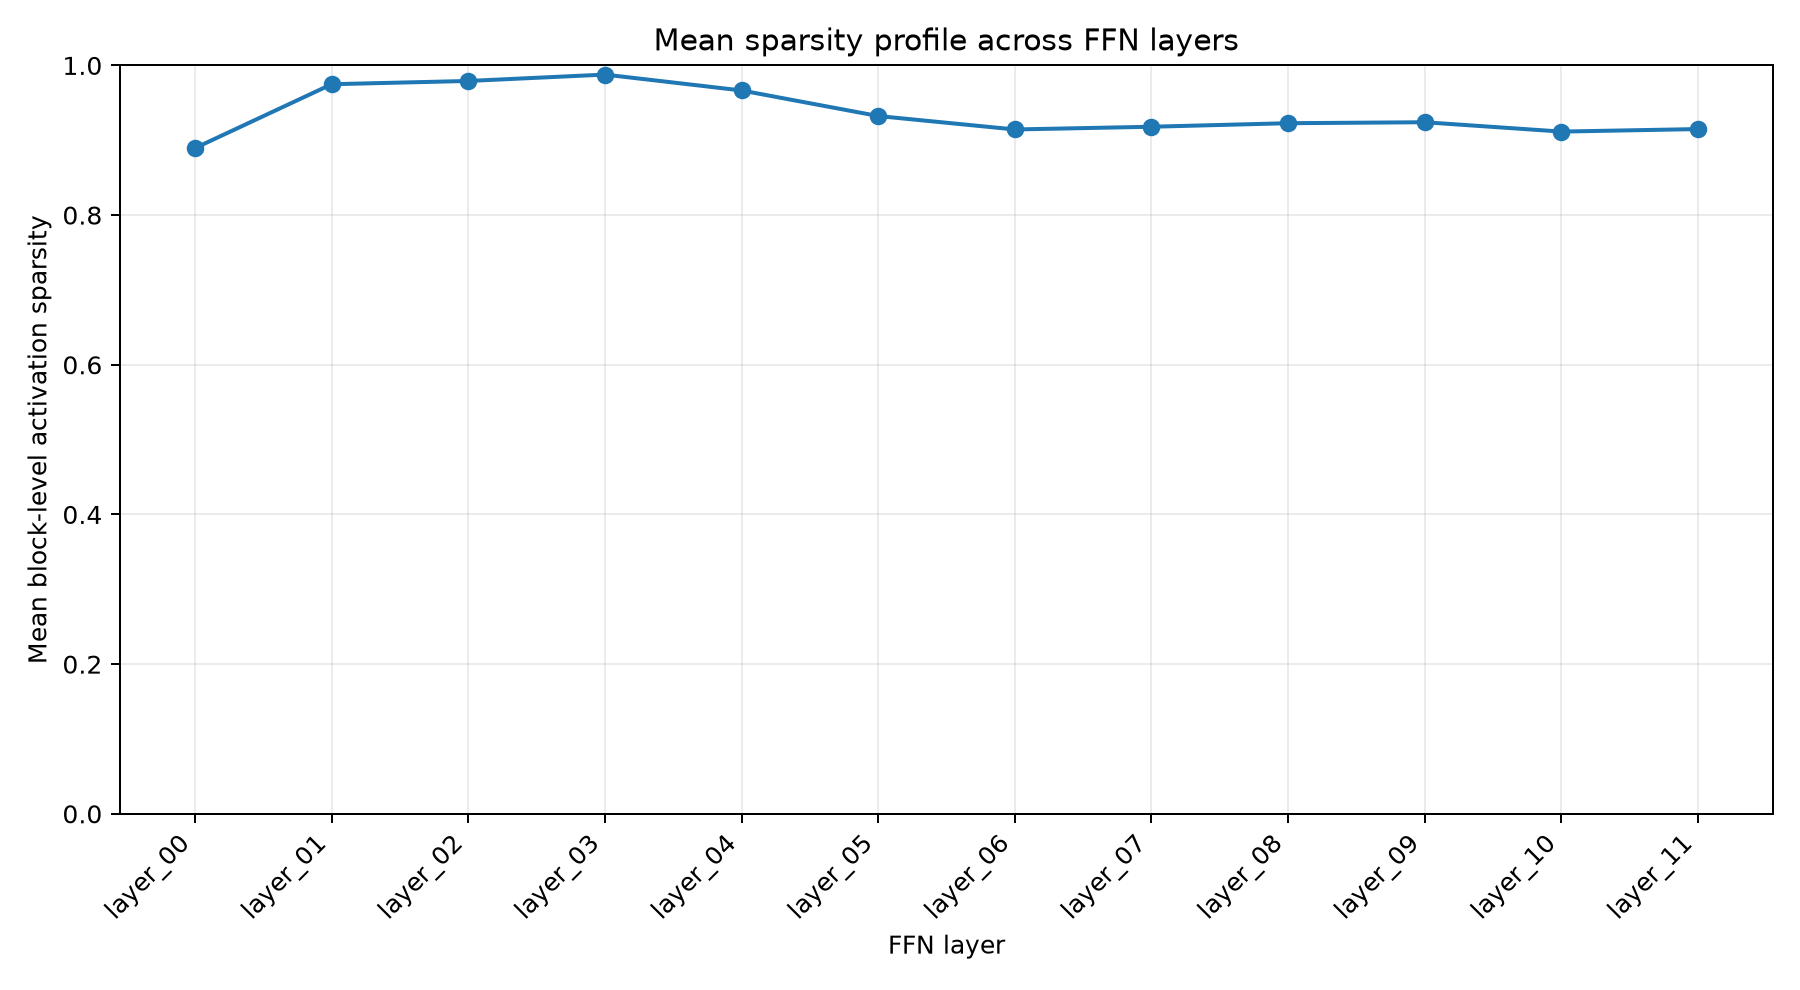
\includegraphics[width=\linewidth,height=4.1cm,keepaspectratio]{assets/rq1_layer_sparsity.png}
\column{.38\textwidth}
\begin{block}{Layer-wise highlights}
\small
\textbf{L0:} 88.96\% sparse $\approx$339 active neurons.\par\vspace{3pt}
\textbf{L3:} \textcolor{Crimson}{\bfseries 98.77\%} sparse $\approx$\textbf{38} active neurons!\par\vspace{3pt}
\textbf{L5:} 93.23\%; \textbf{L6--L11:} 91.2--92.4\%.\par\vspace{3pt}
{\color{Muted}\textit{Non-flat across depth.}}
\end{block}
\end{columns}
\vspace{2pt}
\scriptsize
\begin{tabularx}{\linewidth}{l l l l}
\toprule
Test & Statistic & $p$-value & Decision\\
\midrule
Hotelling contrast  & $T^2=602{,}912.2$               & $1.25\times10^{-57}$ & Reject $\Hnull$\\
RM-ANOVA            & $F=1{,}838.82$; df $(11,429)$    & $<10^{-100}$         & Reject $\Hnull$\\
Greenhouse--Geisser & $\hat\epsilon=0.125$; df $(1.38,53.7)$ & $1.68\times10^{-46}$ & Reject $\Hnull$\\
Friedman            & $Q=432.99$; df $=11$            & $5.99\times10^{-86}$ & Reject $\Hnull$\\
\bottomrule
\end{tabularx}
\vspace{2pt}
\smallnote{Conclusion: sparsity varies significantly with depth. These results do not validate a specific pruning rate or guarantee zero accuracy loss.}
\end{frame}

% =============================================================================
% SLIDE 10 — RQ2 METHOD
% =============================================================================
\begin{frame}{RQ2 | Neuron Co-activation and Functional Modularity — Formulation}
\rqbadge{RQ2}\quad\textbf{Do neurons fire independently or show pairwise dependence?}
\vspace{3pt}
\begin{block}{Null hypothesis}
$\Hnull:\phi_{ij}=0\quad\forall\,i\ne j.$
\end{block}
\begin{columns}[T,onlytextwidth]
\column{.48\textwidth}
\begin{block}{Binary firing indicator and filter}
\begin{equation}
  u_{t,k}=\I(h_{t,k}>0).
  \label{eq:binary_fire}
\end{equation}
Prevalence filter:\quad
$0.01\leq \dfrac{1}{n}\displaystyle\sum_{t}u_{t,k}\leq0.99$.
\end{block}
\column{.49\textwidth}
\begin{block}{Matthews / Phi-correlation}
\begin{equation}
\phi_{ij}=\frac{p_{11}-p_i p_j}
{\sqrt{p_i(1-p_i)\,p_j(1-p_j)}}.
\label{eq:phi_corr}
\end{equation}
$p_i=P(u_i=1)$;\; $p_{11}=P(u_i=1,u_j=1)$.
\end{block}
\end{columns}
\begin{exampleblock}{Hierarchical Agglomerative Clustering (HAC)}
Correlation distance $d_{ij}=1-\phi_{ij}$; Ward's linkage. Cophenetic correlation = \textbf{0.78}.
\end{exampleblock}
\end{frame}

% =============================================================================
% SLIDE 11 — RQ2 RESULTS
% =============================================================================
\begin{frame}{RQ2 | Evidence: Early Co-activation, Deep Decorrelation}
\begin{columns}[T,onlytextwidth]
\column{.60\textwidth}
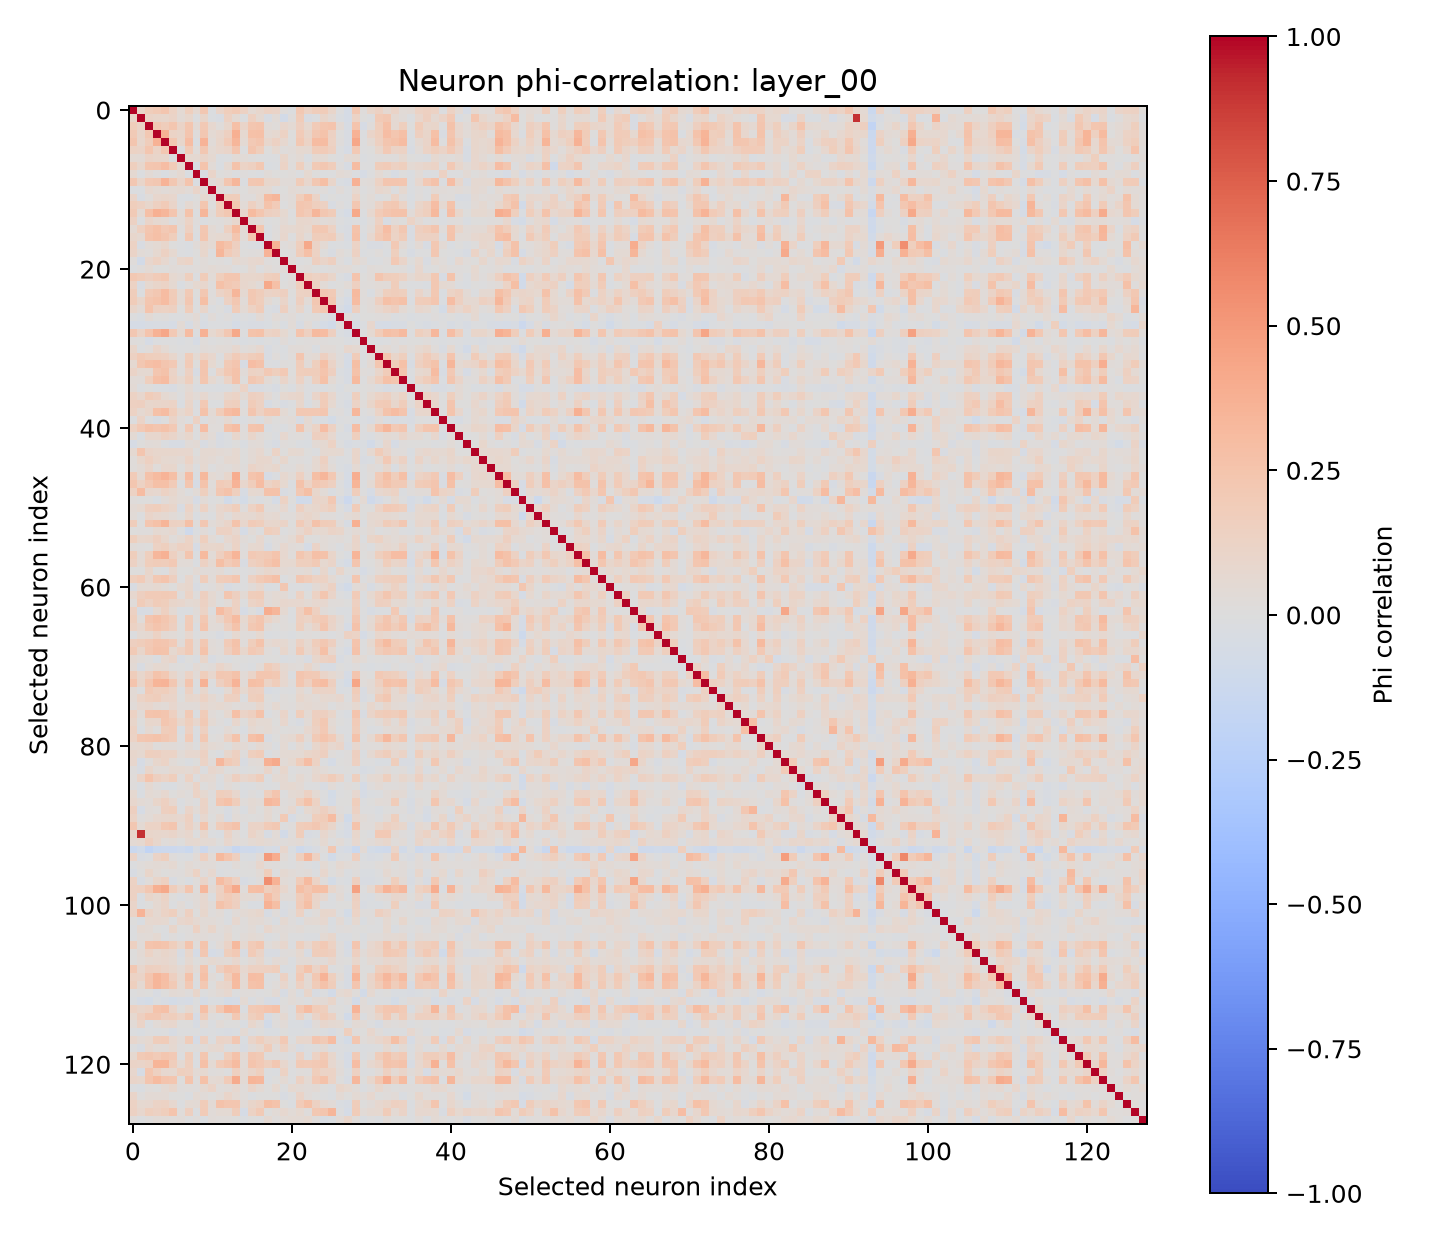
\includegraphics[width=\linewidth,height=3.5cm,keepaspectratio]{assets/rq2_coactivation.png}
\vspace{1pt}
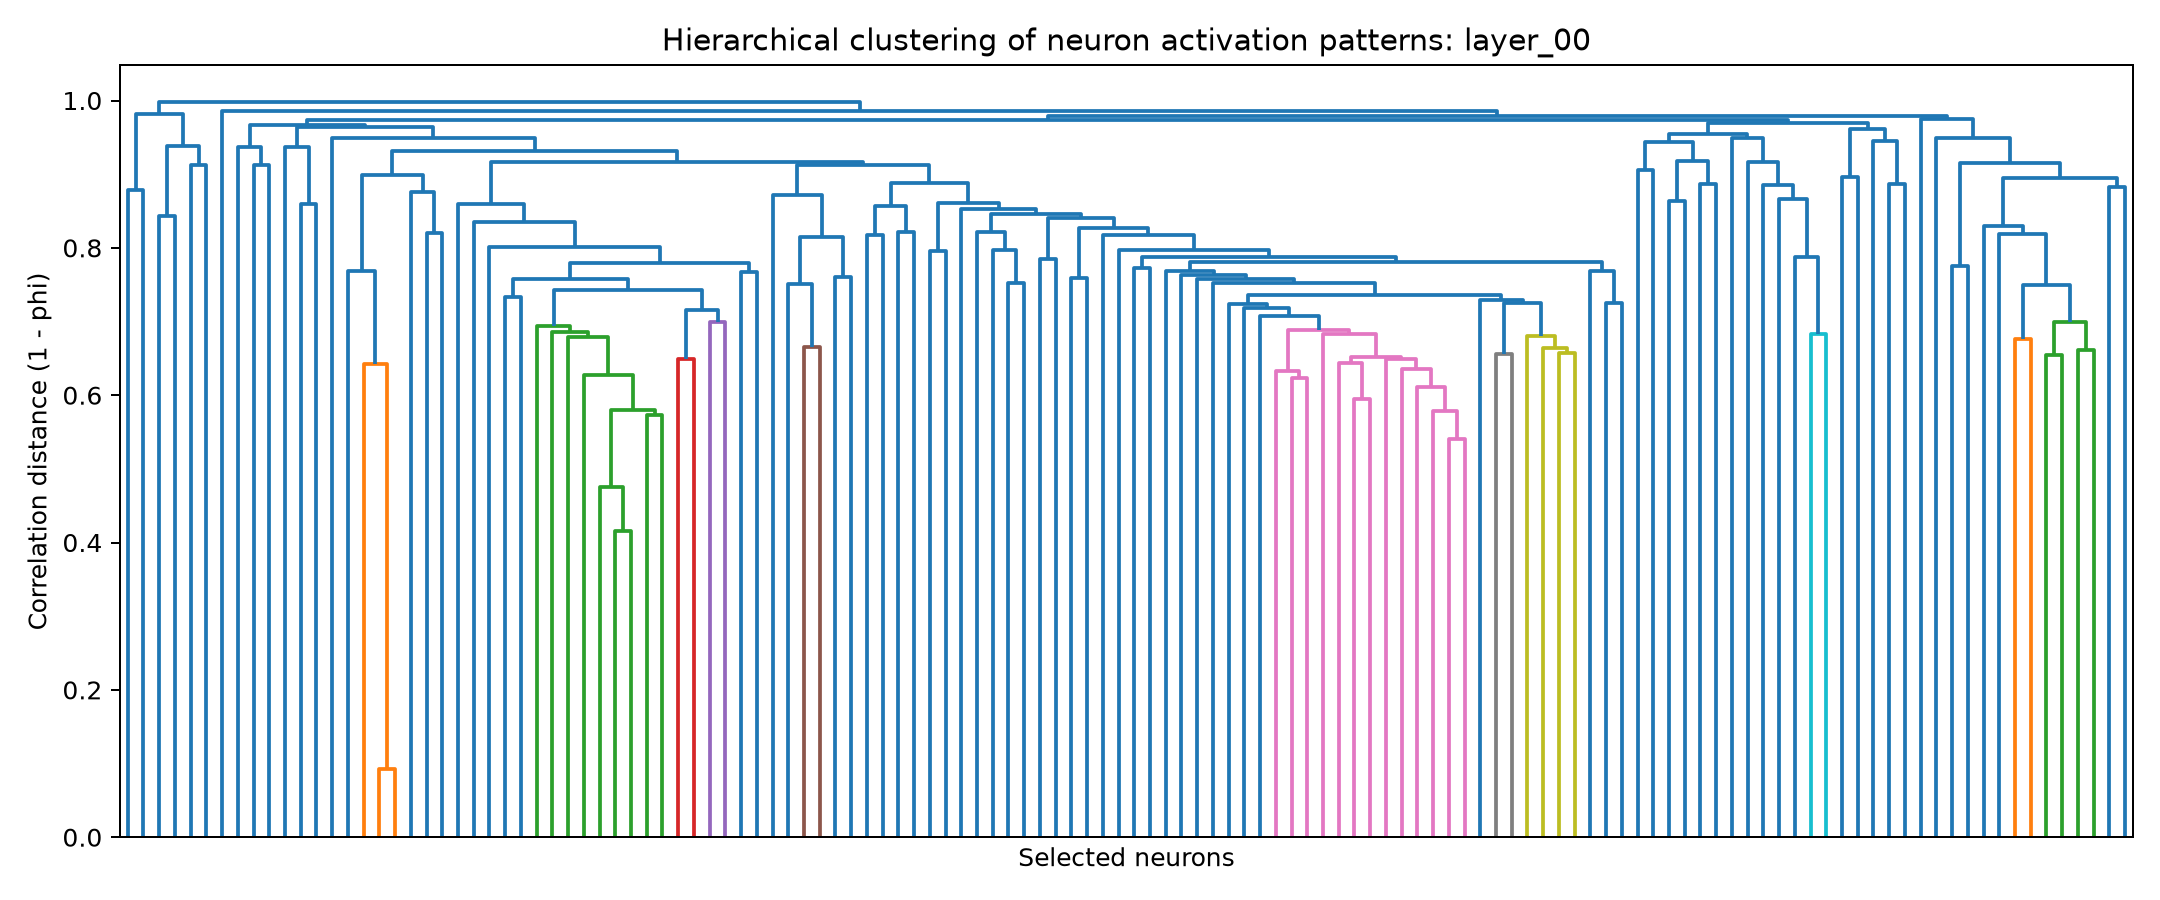
\includegraphics[width=\linewidth,height=1.1cm,keepaspectratio]{assets/rq2_dendrogram.png}
\column{.38\textwidth}
\begin{block}{Layer 0 — coordinated firing}
{\Large\color{NavyMid}\bfseries 76.82\%}\par
{\small positive neuron pairs;\\ mean $\phi=+0.0685$.}
\end{block}
\vspace{3pt}
\begin{block}{Layer 6 — near-zero dependence}
{\Large\color{NavyMid}\bfseries $-0.009$}\par
{\small median $\phi$;\\ $\approx$45\% of pairs positive.}
\end{block}
\vspace{3pt}
\begin{block}{HAC dendogram}
{\small Cophenetic corr.\ = \textbf{0.78};\\ 122/128 clusters at $d=0.70$.}
\end{block}
\end{columns}
\end{frame}

% =============================================================================
% SLIDE 12 — RQ3 METHOD
% =============================================================================
\begin{frame}{RQ3 | Latent Intrinsic Dimensionality — Formulation}
\rqbadge{RQ3}\quad\textbf{How many orthogonal directions carry meaningful variation?}
\begin{block}{Goal}
Quantify effective dimensionality without relying on an arbitrary variance threshold.
\end{block}
\small
\begin{columns}[T,onlytextwidth]
\column{.50\textwidth}
\begin{block}{Participation Ratio (PR)}
Let $\lambda_1\geq\cdots\geq\lambda_m$ be covariance eigenvalues:
\begin{equation}
\PR(S)=\frac{\bigl[\operatorname{tr}(S)\bigr]^2}{\|S\|_F^2}
=\frac{\bigl(\sum_i\lambda_i\bigr)^2}{\sum_i\lambda_i^2}.
\label{eq:PR}
\end{equation}
\end{block}
\column{.49\textwidth}
\begin{block}{Roy--Vetterli Entropy Effective Rank}
\begin{equation}
p_i=\frac{\lambda_i}{\sum_j\lambda_j},\qquad
H=-\sum_i p_i\ln p_i,
\label{eq:entropy}
\end{equation}
\begin{equation}
\erank(S)=\exp(H).
\label{eq:erank}
\end{equation}
\end{block}
\end{columns}
\vspace{3pt}
\small\textbf{Split-half subspace stability:}\quad
$\bar\rho_K=\dfrac{1}{K}\displaystyle\sum_{i=1}^{K}\sigma_i(V_A^T V_B)$,\;
where $\sigma_i$ are singular values of the cross-subspace projection.
\end{frame}

% =============================================================================
% SLIDE 13 — RQ3 RESULTS
% =============================================================================
\begin{frame}{RQ3 | Evidence: Severe Early Collapse, Mid-layer Expansion}
\begin{columns}[T,onlytextwidth]
\column{.52\textwidth}
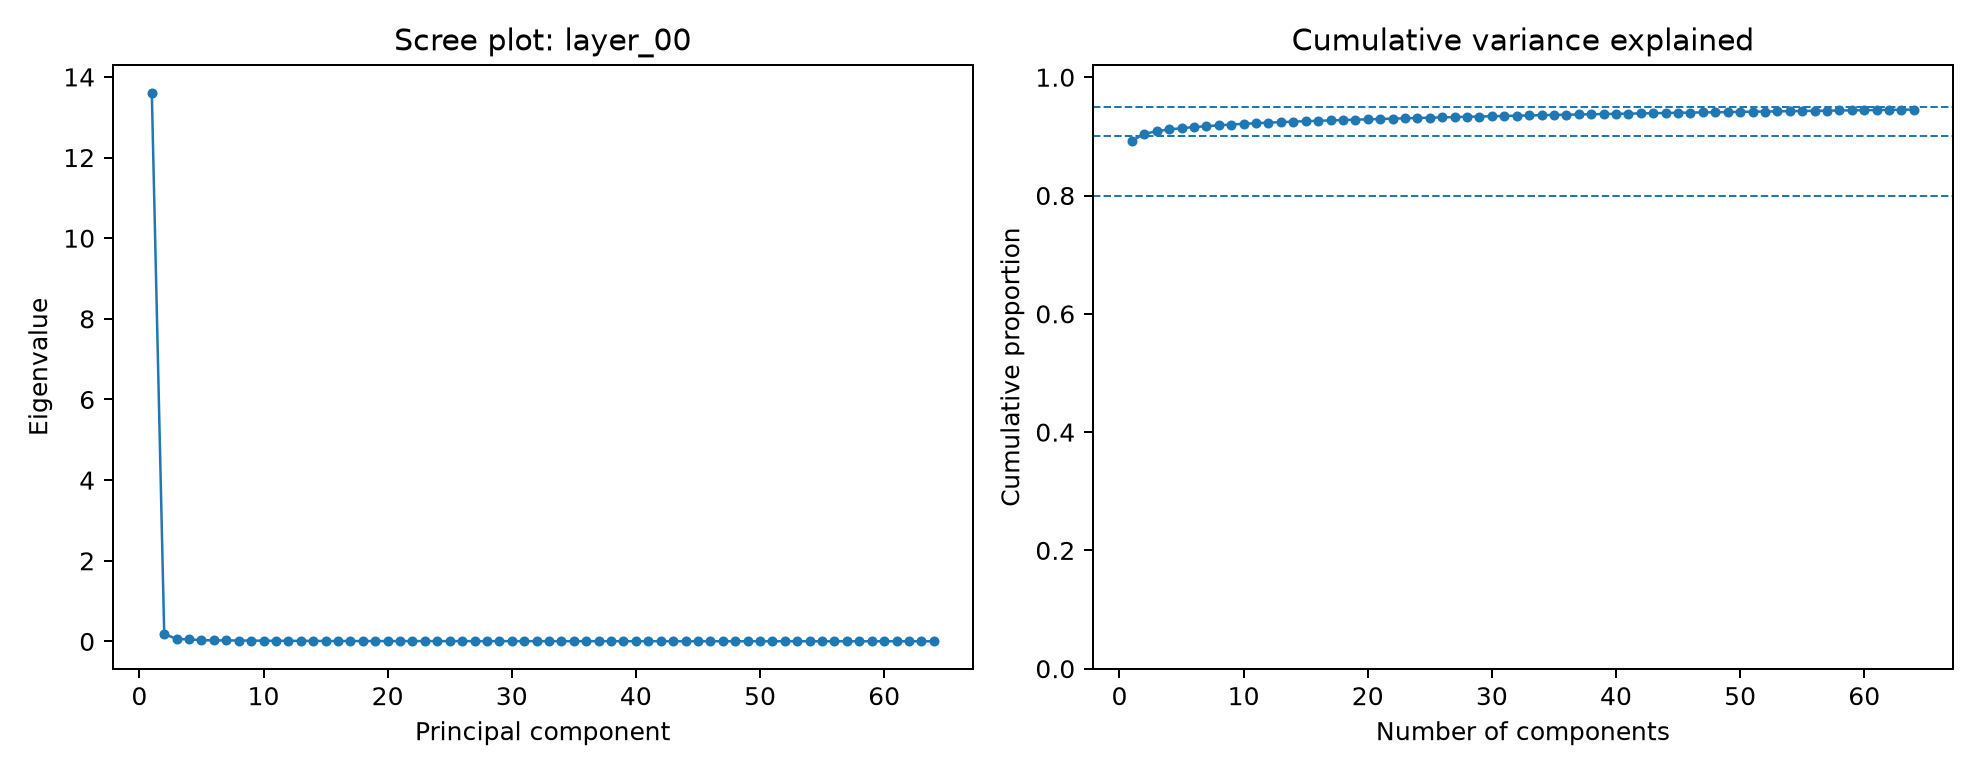
\includegraphics[width=\linewidth,height=3.8cm,keepaspectratio]{assets/rq3_pca.png}
\vspace{2pt}
\begin{block}{Layer 0 (extreme collapse)}
{\large\color{NavyMid}\bfseries 81.4\%} variance in PC1 alone;\quad PR$=1.12$,\; erank$=1.51$.
\end{block}
\column{.46\textwidth}
\scriptsize
\begin{tabular}{lrrr}
\toprule
Layer & PR & erank & Stability $K=5$\\
\midrule
L0  &  1.12 &  1.51 & 0.894\\
L1  &  3.89 & 13.06 & 0.963\\
L2  &  1.20 &  1.86 & 0.986\\
L3  &  2.45 &  7.72 & 0.972\\
L4  &  3.51 & 12.19 & 0.977\\
L5  & 31.40 & 46.36 & 0.948\\
L6  & 29.86 & 45.53 & 0.964\\
L7  & 30.99 & 45.98 & 0.869\\
L8  & 31.42 & 46.10 & 0.976\\
L9  & 29.64 & 44.03 & 0.984\\
L10 & 27.64 & 41.43 & 0.971\\
L11 &  3.38 & 10.81 & 0.986\\
\bottomrule
\end{tabular}
\vspace{2pt}
\smallnote{PR and erank are distinct measures. Middle-layer entropy rank $\approx$41--46; split-half stability $>0.86$ throughout.}
\end{columns}
\end{frame}

% =============================================================================
% SLIDE 14 — RQ4 METHOD
% =============================================================================
\begin{frame}{RQ4 | Static Weight Rank vs.\ Dynamic Activation Rank — Formulation}
\rqbadge{RQ4}\quad\textbf{Is weight spectral capacity a reliable proxy for activation dimensionality?}
\begin{block}{Goal}
Compare layer-wise entropy effective rank of weight matrices ($\erank_W$) with that of token activation matrices ($\erank_A$).
\end{block}
\small
\begin{columns}[T,onlytextwidth]
\column{.49\textwidth}
\begin{block}{Singular Value Decomposition}
\begin{equation}
W=U\Sigma V^T,\qquad
p_{i,W}=\frac{\sigma_i^2}{\sum_j\sigma_j^2}.
\label{eq:svd}
\end{equation}
\begin{equation}
\erank_W=\exp\!\Bigl(-\sum_i p_{i,W}\ln p_{i,W}\Bigr).
\label{eq:erank_W}
\end{equation}
\end{block}
\column{.49\textwidth}
\begin{block}{Activation effective rank}
\begin{equation}
p_{i,A}=\frac{\lambda_i}{\sum_j\lambda_j},
\label{eq:erank_A_p}
\end{equation}
\begin{equation}
\erank_A=\exp\!\Bigl(-\sum_i p_{i,A}\ln p_{i,A}\Bigr).
\label{eq:erank_A}
\end{equation}
Pearson $r$ and Spearman $\rho$ across 12 layers.
\end{block}
\end{columns}
\vspace{2pt}
\smallnote{OPT-125M: fc1 is $3072\times768$; fc2 is $768\times3072$. Each matrix has at most 768 singular values.}
\end{frame}

% =============================================================================
% SLIDE 15 — RQ4 RESULTS
% =============================================================================
\begin{frame}{RQ4 | Evidence: Weight Capacity and Activation Geometry Decouple}
\begin{columns}[T,onlytextwidth]
\column{.56\textwidth}
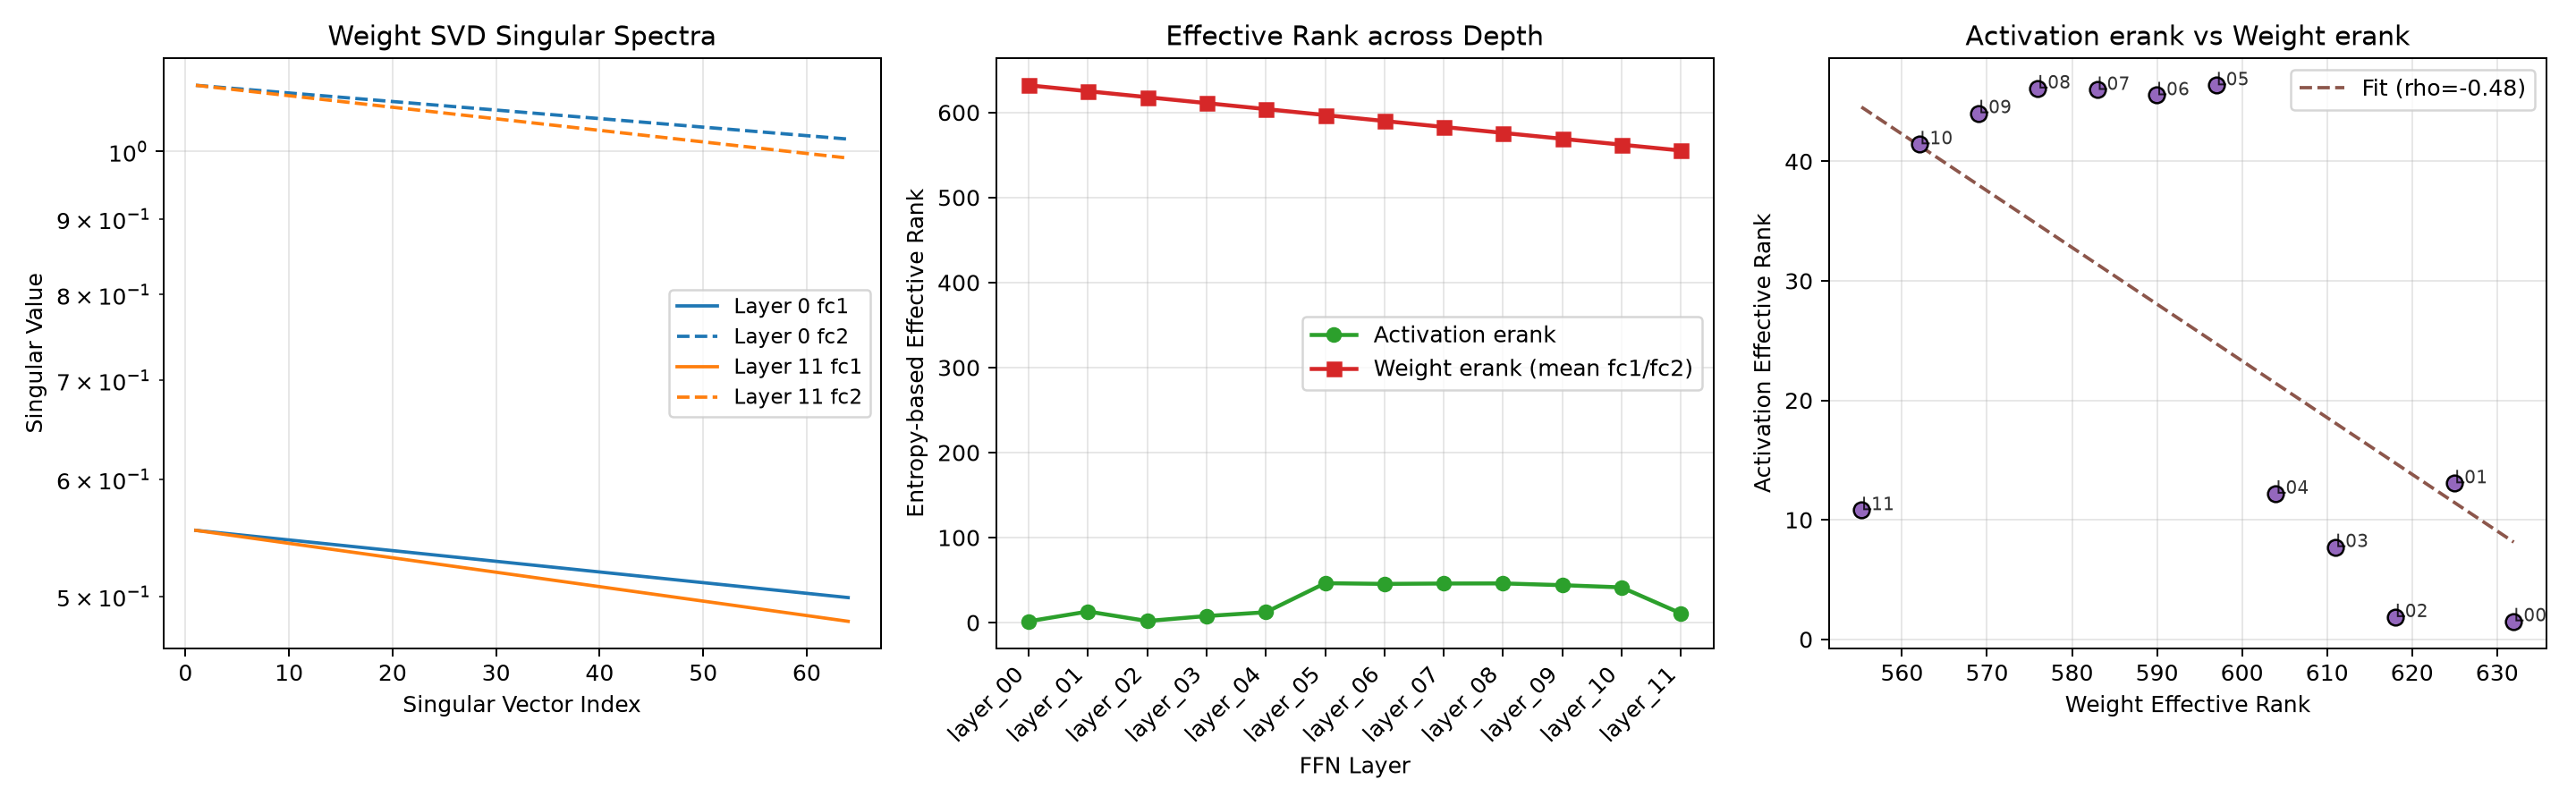
\includegraphics[width=\linewidth,height=3.2cm,keepaspectratio]{assets/rq4_weight_activation.png}
\column{.42\textwidth}
\begin{block}{Effective-rank comparison}
\small
\textbf{Mean weight rank:}\quad $\erank_W=593.51$\\
(out of maximum 768).\par\vspace{4pt}
\textbf{Mean activation rank:}\quad $\erank_A=26.10$\\
(out of nominal $d_{ff}=3{,}072$).\par\vspace{4pt}
\textbf{Rank-scale mismatch:}\quad ${\approx}23\times$.
\end{block}
\end{columns}
\vspace{2pt}
\scriptsize
\begin{tabularx}{\linewidth}{X r r}
\toprule
Association measure & Coefficient & $p$-value\\
\midrule
Pearson, entropy effective rank    & $r=-0.607$   & 0.036 \\
Spearman, entropy effective rank   & $\rho=-0.622$& 0.031 \\
Pearson, participation ratio       & $r=-0.592$   & 0.042 \\
\bottomrule
\end{tabularx}
\vspace{2pt}
\smallnote{Pearson associations are significant at the 5\% level; the \emph{negative} sign means higher weight rank corresponds to lower activation rank — not direct coupling.}
\end{frame}

% =============================================================================
% SLIDE 16 — RQ5 METHOD
% =============================================================================
\begin{frame}{RQ5 | Cross-Domain Representation Invariance — Formulation}
\rqbadge{RQ5}\quad\textbf{Are FFN activation manifolds invariant across text domains?}
\begin{block}{Null hypothesis}
\begin{equation}
\Hnull:\boldsymbol\mu_{\mathrm{wiki}}=\boldsymbol\mu_{\mathrm{sci}}=\boldsymbol\mu_{\mathrm{news}}.
\label{eq:rq5_H0}
\end{equation}
\end{block}
\small
\begin{columns}[T,onlytextwidth]
\column{.50\textwidth}
\begin{block}{MANOVA between/within decomposition}
\begin{equation}
T=H+E,\quad
H=\sum_{g}n_g(\bar{x}_g-\bar{x})(\bar{x}_g-\bar{x})^T.
\label{eq:manova}
\end{equation}
\end{block}
\column{.47\textwidth}
\begin{block}{Wilks' $\Lambda$ and Pillai's Trace}
Let $\xi_i$ be eigenvalues of $E^{-1}H$:
\begin{equation}
\Lambda=\prod_i\frac{1}{1+\xi_i},
\qquad
V=\sum_i\frac{\xi_i}{1+\xi_i}.
\label{eq:wilks_pillai}
\end{equation}
\end{block}
\end{columns}
\vspace{2pt}
\smallnote{Box's $M$ tests $H_0:\Sigma_1=\Sigma_2=\Sigma_3$; LDA evaluates discriminability of projected activation coordinates across domain labels.}
\end{frame}

% =============================================================================
% SLIDE 17 — RQ5 RESULTS
% =============================================================================
\begin{frame}{RQ5 | Evidence: Activation Manifolds Encode Text Domain}
\begin{columns}[T,onlytextwidth]
\column{.52\textwidth}
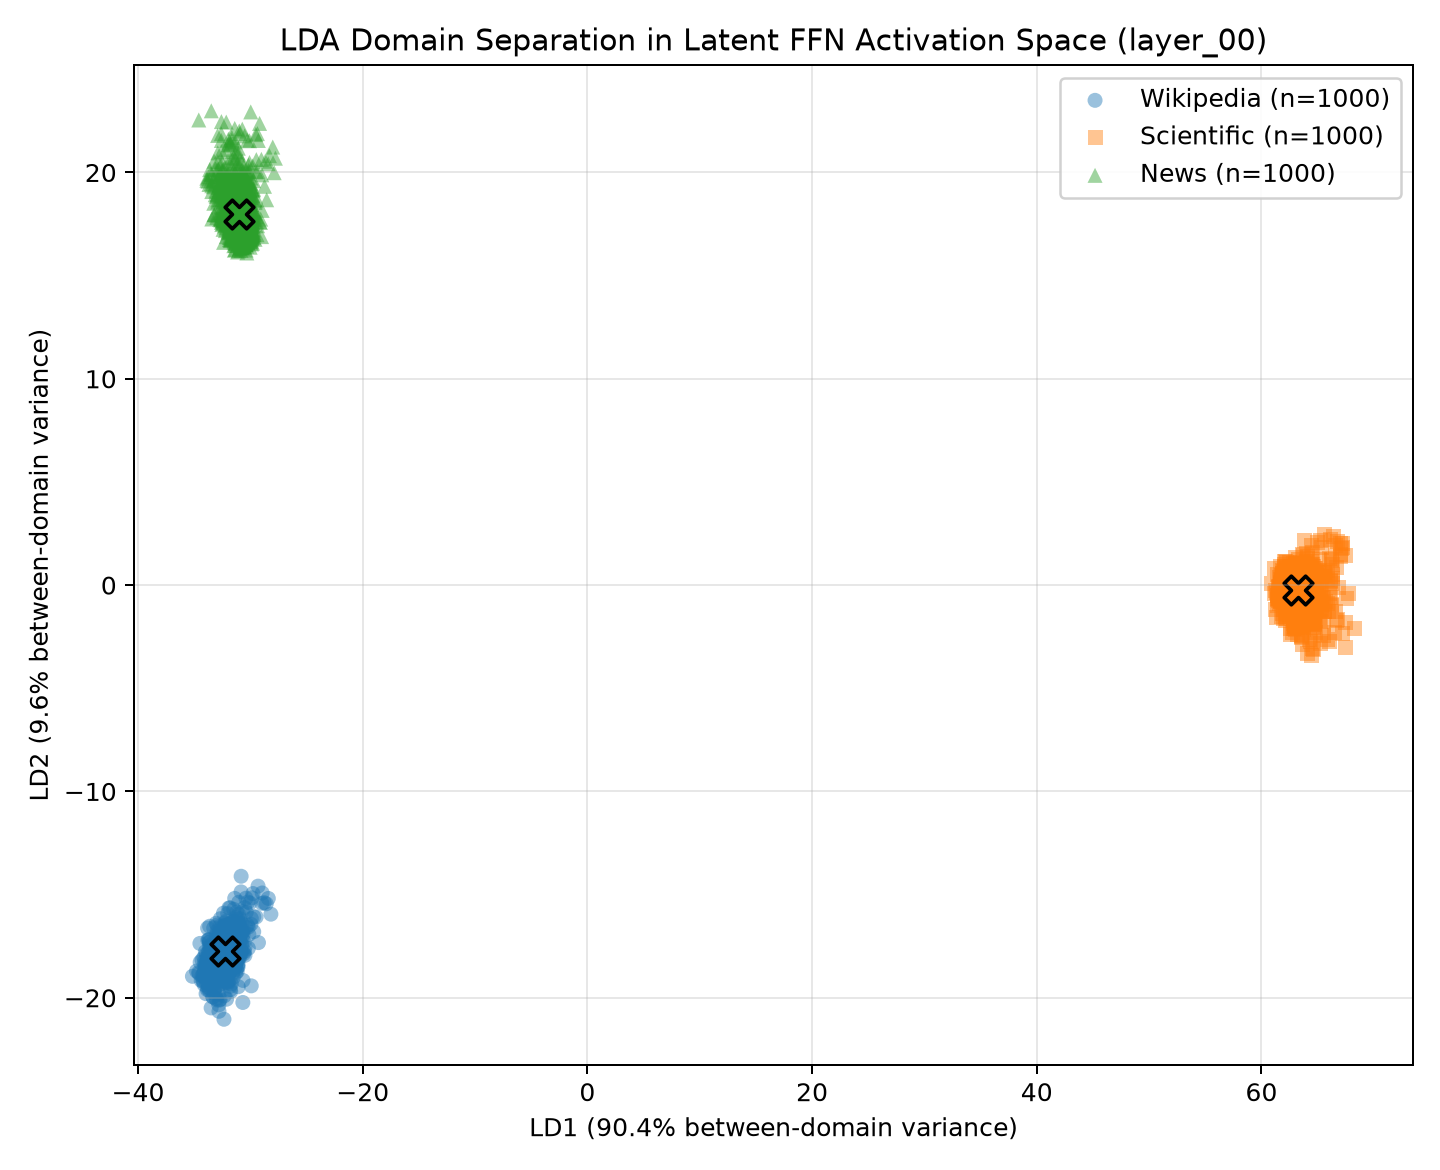
\includegraphics[width=\linewidth,height=3.2cm,keepaspectratio]{assets/rq5_lda.png}
\column{.46\textwidth}
\begin{block}{Key results}
\small
\textbf{Wilks' $\Lambda$:} $2.33\times10^{-6}$.\par\vspace{3pt}
\textbf{Pillai's Trace:} $1.84$.\par\vspace{3pt}
\textbf{5-fold CV LDA accuracy:} \textcolor{NavyMid}{\bfseries 100.0\%}\\
{\footnotesize(chance baseline: 33.3\%, 3-class).}
\end{block}
\end{columns}
\vspace{2pt}
\scriptsize
\begin{tabularx}{\linewidth}{X l l}
\toprule
Test / metric & Reported result & Decision\\
\midrule
One-way MANOVA       & Wilks $F(16,178)=153.21$; $p=0.000$        & Reject $\Hnull$\\
Pillai's Trace test  & $V=1.84$; $p=0.000$                        & Reject $\Hnull$\\
Box's $M$            & $M=15{,}693.7$; $F(72,11442)=207.12$; $p=0.000$ & Reject $\Sigma_g$ equality\\
Pairwise Hotelling   & All pairs: $T^2>5.9\times10^5$              & All pairs separable\\
5-fold CV LDA        & Accuracy = 100.0\%; SD = 0.00               & Domains discriminable\\
\bottomrule
\end{tabularx}
\vspace{2pt}
\smallnote{$p=0.000$ reflects numerical output precision, not an exact probability of zero. Domain-aware routing is a proposed, not implemented, application.}
\end{frame}

% =============================================================================
% SLIDE 18 — MASTER SYNTHESIS MATRIX
% =============================================================================
\begin{frame}{Master Summary Matrix: What the Five RQs Establish}
\scriptsize
\begin{tabularx}{\linewidth}{>{\bfseries}p{0.055\linewidth} p{0.19\linewidth} p{0.33\linewidth} X}
\toprule
RQ & Target & Key Empirical Evidence & Architectural Conclusion\\
\midrule
RQ1 & Sparsity flatness &
  L3 = 98.77\%; GG $p=1.68\times10^{-46}$; Friedman $p=5.99\times10^{-86}$ &
  Sparsity changes with depth; a single threshold is not supported.\\[3pt]
RQ2 & Neuron independence &
  L0 mean $\phi=+0.0685$; L6 median $\phi=-0.009$; 122/128 clusters &
  Early co-activation weakens substantially with depth.\\[3pt]
RQ3 & Full-rank latent space &
  L0 PR$=1.12$, erank$=1.51$; L5--L10 erank $\approx$41--46; stability $>0.86$ &
  Activations occupy a compact, repeatable subspace.\\[3pt]
RQ4 & Weight/activation coupling &
  $\erank_W=593.51$ vs $\erank_A=26.10$; Pearson $r=-0.607$, $p=0.036$ &
  Static weight spectrum is not a proxy for dynamic rank.\\[3pt]
RQ5 & Domain invariance &
  Wilks $\Lambda=2.33\times10^{-6}$; Box's $M=15{,}693.7$; LDA$=100\%$ &
  Activations carry strong domain-specific statistical signatures.\\
\bottomrule
\end{tabularx}
\vspace{5pt}
\takeaway{Across all five questions, the common pattern is \emph{structured sparsity}: it varies by layer, by neuron pair, by latent direction, and by text domain.}
\end{frame}

% =============================================================================
% SLIDE 19 — ARCHITECTURAL INTERPRETATION
% =============================================================================
\begin{frame}{Architectural Interpretation Across Network Depth}
\centering
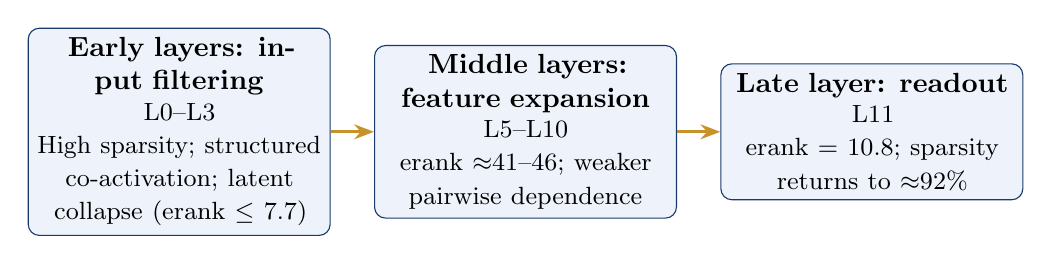
\begin{tikzpicture}[
  phase/.style={rounded corners=4pt,draw=NavyMid,fill=IceBlue,
                minimum height=1.55cm,text width=3.6cm,align=center},
  arr/.style={-{Stealth[length=2.5mm]},very thick,color=Gold}
]
\node[phase] (early) {%
  \textbf{Early layers: input filtering}\\
  \small L0--L3\\
  High sparsity; structured co-activation; latent collapse (erank $\leq7.7$)};
\node[phase,right=0.55cm of early] (middle) {%
  \textbf{Middle layers: feature expansion}\\
  \small L5--L10\\
  erank $\approx$41--46; weaker pairwise dependence};
\node[phase,right=0.55cm of middle] (late) {%
  \textbf{Late layer: readout}\\
  \small L11\\
  erank $=10.8$; sparsity returns to $\approx$92\%};
\draw[arr] (early)--(middle); \draw[arr] (middle)--(late);
\end{tikzpicture}
\vspace{0.5cm}
\begin{columns}[T,onlytextwidth]
\column{.32\textwidth}
\begin{block}{Layer sparsity profile}
Non-flat; strongest peak at Layer 3 (98.77\%).
\end{block}
\column{.32\textwidth}
\begin{block}{Neuron structure}
Co-activation clusters clearer in L0 than in L6.
\end{block}
\column{.32\textwidth}
\begin{block}{Latent geometry}
Rank expands in middle layers; not set by weight rank alone.
\end{block}
\end{columns}
\smallnote{This slide summarises empirical patterns; it does not assert causal semantic roles for individual layers.}
\end{frame}

% =============================================================================
% SLIDE 20 — ENGINEERING IMPLICATIONS
% =============================================================================
\begin{frame}{Engineering Implications and Research Opportunities}
\begin{columns}[T,onlytextwidth]
\column{.49\textwidth}
\begin{block}{Supported by the results}
\begin{itemize}
  \item Explore \emph{layer-adaptive} rather than uniform sparsity policies.
  \item Evaluate sparse kernels where zero fractions are high ($>90\%$).
  \item Investigate low-rank approximations for layers with compact geometry.
  \item Avoid using static weight rank as a stand-alone proxy for activation rank.
\end{itemize}
\end{block}
\column{.49\textwidth}
\begin{alertblock}{Promising extensions (not implemented here)}
\begin{itemize}
  \item Domain-conditioned routing using learned activation features.
  \item Specialist FFN experts for scientific, news and encyclopedic text.
  \item Hardware-level profiling of sparse/low-rank execution.
  \item Accuracy-preserving pruning and reconstruction ablations.
\end{itemize}
\end{alertblock}
\end{columns}
\takeaway{The statistics motivate targeted compression experiments. Any claim of zero accuracy loss or measured speed-up requires a separate intervention study.}
\end{frame}

% =============================================================================
% SLIDE 21 — LIMITATIONS AND FUTURE WORK
% =============================================================================
\begin{frame}{Limitations and Future Directions}
\begin{columns}[T,onlytextwidth]
\column{.48\textwidth}
\begin{block}{Current limitations}
\begin{itemize}
  \item Single frozen model: OPT-125M only.
  \item Primary analysis uses WikiText-2.
  \item ReLU gives exact zeros; results may not transfer to GELU or SwiGLU activations.
  \item Domain tests use a reduced $K=8$ PCA space for stable covariance estimation.
  \item Statistics are observational, not causal tests.
\end{itemize}
\end{block}
\column{.49\textwidth}
\begin{exampleblock}{Future directions}
\begin{itemize}
  \item Scale to larger Transformers (OPT-1.3B, LLaMA) and diverse benchmarks.
  \item Compare ReLU, GELU, and SwiGLU activation families.
  \item Test pruning and low-rank reconstruction against held-out perplexity.
  \item Evaluate sparse inference on real hardware (GPU/accelerators).
  \item Study runtime domain-aware routing and its overhead.
\end{itemize}
\end{exampleblock}
\end{columns}
\end{frame}

% =============================================================================
% SLIDE 22 — CONCLUSION
% =============================================================================
\begin{frame}{Conclusion}
\begin{block}{What this project contributes}
A multivariate statistical characterisation of post-ReLU FFN activations across all 12 layers of OPT-125M, combining profile analysis (RM-ANOVA, Friedman), binary dependence ($\phi$-correlation, HAC), PCA/effective rank, weight SVD, and cross-domain MANOVA/LDA.
\end{block}
\begin{enumerate}
  \item Sparsity is strongly depth-dependent, with a \textbf{98.77\%} peak at Layer 3.
  \item Early-layer neuron co-activation (mean $\phi=+0.069$) weakens substantially by Layer 6.
  \item Activation variation concentrates in a compact latent subspace (erank $\leq46$, not 3,072).
  \item Dense weight matrices remain high-rank ($\erank_W\approx594$) while activations are low-rank ($\erank_A\approx26$).
  \item FFN activation distributions discriminate text domains with 100\% LDA accuracy.
\end{enumerate}
\vspace{3pt}
\takeaway{The key finding is not simply that FFN activations are sparse: their sparsity, dependence structure, and intrinsic dimensionality are \emph{organised} and vary systematically with both network depth and input domain.}
\end{frame}

% =============================================================================
% APPENDIX
% =============================================================================
\appendix

% SLIDE A1 — Numerical reconciliation note
\begin{frame}{Appendix A | Statistical Values Reference}
\small
The main slides use values from the final project report (Tables 4.1--4.5).
\vspace{3pt}
\scriptsize
\begin{tabularx}{\linewidth}{p{0.10\linewidth} X X}
\toprule
Area & Summary / earlier deck & Report values used in this presentation\\
\midrule
RQ1 RM-ANOVA   & $F(11,209)=176.43$; GG df $(1.38,26.2)$          & $F=1{,}838.82$, df $(11,429)$; GG df $(1.38,53.7)$; $p_{GG}=1.68\times10^{-46}$\\
RQ2 Layer 6    & Median $\phi=-0.009$                              & Median $\phi=-0.009$ (also reported as $-0.0047$; use report table value)\\
RQ3 Layer 0    & PR reported as 1.51                               & PR$=1.12$; entropy effective rank $=1.51$ (two distinct measures)\\
RQ4 Spearman   & $\rho=-0.622$, $p=0.031$                          & Pearson $r=-0.607$ ($p=0.036$); Spearman $\rho=-0.622$ ($p=0.031$) both listed\\
RQ5 MANOVA     & $F(16,178)=153.21$; Pillai$=1.84$                 & Wilks $F(16,178)=153.21$; Pillai$=1.84$ used here\\
\bottomrule
\end{tabularx}
\vspace{5pt}
\begin{alertblock}{Verify before final defence}
If any value comes from a newer experimental rerun, update the report and all tables consistently. Do not mix test statistics from different runs or label entropy effective rank as Participation Ratio.
\end{alertblock}
\end{frame}

% SLIDE A2 — References and Thank You
\begin{frame}{References and Discussion}
\small
\begin{enumerate}
  \item M. Geva, R. Schuster, J. Berant and O. Levy, ``Transformer Feed-Forward Layers Are Key-Value Memories,'' \emph{EMNLP}, 2021.
  \item Z. Li, C. Wang, Y. Gu, C. Liu and J. Chen, ``On Emergence of Activation Sparsity in Trained Transformers,'' \emph{ICLR}, 2023.
  \item R. A. Johnson and D. W. Wichern, \emph{Applied Multivariate Statistical Analysis}, 6th ed., Pearson, 2014.
  \item O. Roy and M. Vetterli, ``The Effective Rank: A Measure of Effective Dimensionality,'' \emph{EUSIPCO}, pp. 606--610, 2007.
  \item W. K. H\"ardle and L. Simar, \emph{Applied Multivariate Statistical Analysis}, Springer, 2019.
\end{enumerate}
\vspace{0.4cm}
\begin{center}
{\color{NavyMid}\Huge\bfseries Thank You!}\\[6pt]
{\Large Questions \& Discussion}\\[0.6cm]
{\normalsize Lakshmi Ganapathi Kodi (BT23MA005)
  \quad$\mid$\quad Saurabh Kumar Gupta (BT23MA006)}\\[3pt]
{\small Under the guidance of Prof.\ Ashis SenGupta (ISI Kolkata)
  \quad$\mid$\quad Dr. C Lalengmawia (NIT Mizoram)}
\end{center}
\end{frame}

\end{document}
